\documentclass[11pt]{beamer}

\usepackage[utf8]{inputenc}
\usepackage[spanish]{babel}
\usepackage{amsmath}
\usepackage{cancel}
\usepackage{graphicx}
\usepackage{subfig}
\usepackage{caption}
\usepackage{lipsum}
\usepackage{lipsum}
\usepackage{mathtools}
\usepackage{amssymb}
\usepackage{xcolor}


\title{Almacenamiento de memoria en redes de Hopfield}
\author{Julián López Carballal, Jorge García Beni, Rubén de San Juan Morales, Fernando García Sánchez y José Luis Miranda Mora}
\date{\vspace{0cm}}

\begin{document}
	
\frame{\titlepage}

\begin{frame}
\frametitle{Red de Hopfield}
\begin{itemize}
	\item Red formada por $N$ neuronas.
	\item Estados $\sigma_i(t)=\pm 1$.
	\item Evolución temporal discreta con pasos $\Delta t$.
	\item Interaccionan con pesos $J_{ij}$.
	\begin{displaymath}
	\Phi_i(t)=\sum_{j\neq i} J_{ij}\sigma_j
	\end{displaymath}
	\item Su fin: almacenamiento y reproducción de patrones.
	\begin{displaymath}
	\mathcal{P}^\mu_i = \pm1, \,i \in[1,N],\,\mu\in[1,K]\Rightarrow\frac{1}{N}\sum_{i=1}^N \mathcal{P}^\mu_i \mathcal{P}^\nu_i = \delta^{\mu\nu}
	\end{displaymath}
	Patrón reproducido si $\sigma_i(t)=\sigma_i(t+\Delta t)=\mathcal{P}^\mu_i$.
\end{itemize}
\end{frame}

\begin{frame}
\frametitle{Red de Hopfield}
\framesubtitle{Analogía con el modelo de Ising}
\begin{itemize}
	\item Red de Hopfield $\sim$ Modelo de Ising para sistemas magnéticos.
	\item Hamiltoniano $\equiv$ Ising ($\vec{B}=0$).
	\begin{displaymath}
	H = -\frac{1}{2}\sum_{i}\sum_{j\neq i}J_{ij}\sigma_i\sigma_j
	\end{displaymath}
	imponemos $J_{ij}=J_{ji}$.
\end{itemize}
\end{frame}

\begin{frame}
\frametitle{Red de Hopfield}
\begin{itemize}
	\item Solapamiento: cuantificación de la coincidencia con el patrón.
	\begin{displaymath}
	m^\mu(t)=\frac{1}{N}\sum_i \mathcal{P}^\mu_i\sigma_i(t)
	\label{overlap}
	\end{displaymath}
	valor máximo $m^\mu=1$ cuando el patrón es replicado.
	\item Elegimos los pesos:
	\begin{displaymath}
	J_{ij}=\frac{1}{N}\sum_{\mu=1}^K \mathcal{P}^\mu_i \mathcal{P}^\mu_j
	\end{displaymath}
	relacionan espines con el patrón.
\end{itemize}
\end{frame}

\begin{frame}
\frametitle{Generalización del modelo de Hopfield}
\begin{itemize}
	\item Hasta ahora hemos tratado un sistema sin ruido.
	\item En un sistema con ruido se pueden llegar a estados fuera de la dinámica que tratamos.
	\item Introducimos el ruido en forma de una temperatura efectiva $T$.
	\item Adopta la dinámica de espines de Glauber. La distribución se relaja a la de Gibbs:
	\begin{displaymath}
	P(\lbrace\sigma\rbrace)\propto e^{-H(\lbrace\sigma\rbrace)/T}
	\end{displaymath}
	este es el \textbf{modelo de Hopfield generalizado}.
\end{itemize}
\end{frame}

\begin{frame}
\frametitle{Generalización del modelo de Hopfield}
\framesubtitle{Teoría de campo medio}
\begin{itemize}
	\item Tomamos unidades $k_B=1$.
	\item Densidad de energía libre:
	\begin{displaymath}
	f(T)=-\frac{T}{N}\left<\log Z\right>_{\mathcal{P}}
	\end{displaymath}
	\item Función de partición:
	\begin{displaymath}
	\hspace{-1.225cm}Z=\left(\frac{N}{T}\right)^{\frac{K}{2}}e^{-\frac{K}{2T}}\int\prod_\mu \frac{dm^\mu}{\sqrt{2\pi}}\exp\Bigg\{-\frac{N\vec{m}^2}{2T}+\sum_i \log\left[2\cosh\left(\frac{\vec{m}\cdot\vec{\mathcal{P}_i}}{T}\right)\right]\Bigg\}
	\end{displaymath}
\end{itemize}
\end{frame}

\begin{frame}
\frametitle{Generalización del modelo de Hopfield}
\framesubtitle{Teoría de campo medio}
\begin{itemize}
	\item Si K es finito:
	\begin{displaymath}
	-\frac{T\ln Z}{N}=\frac{1}{2}\vec{m}^2-\frac{T}{N}\sum_i\ln\left[2\cosh\left(\frac{\vec{m}\cdot\vec{\mathcal{P}_i}}{T}\right)\right]
	\end{displaymath}
	\item El parámetro de orden viene dado por la ecuación $\partial\ln Z/\partial m^\mu$=0:
	\begin{displaymath}
	\vec{m}=\frac{1}{N}\sum_i \vec{\mathcal{P}_i}\tanh\left(\frac{\vec{m}\cdot\vec{\mathcal{P}_i}}{T}\right)
	\end{displaymath}
	\item En LT: $(1/N)\sum_i$ $\rightarrow$ promedios sobre $\lbrace\vec{\mathcal{P}_i}\rbrace$.
\end{itemize}
\end{frame}

\begin{frame}
\frametitle{Generalización del modelo de Hopfield}
\framesubtitle{Teoría de campo medio}
\begin{itemize}
	\item Ecuaciones de campo medio:
	\begin{displaymath}
	f(T)=\frac{1}{2}\vec{m}^2 - T\left<\log\left[2\cosh\left(\frac{\vec{m}\cdot\vec{\mathcal{P}_i}}{T}\right)\right]\right>_{\mathcal{P}}
	\end{displaymath}
	\begin{displaymath}
	\vec{m}=\left<\vec{\mathcal{P}_i}\cdot\tanh\left(\frac{\vec{m}\cdot\vec{\mathcal{P}_i}}{T}\right)\right>_{\mathcal{P}}
	\end{displaymath}
	\item Promedio térmico de los espines: $\left<\sigma_i\right>=\tanh\left(\frac{\vec{m}\cdot\vec{\mathcal{P}_i}}{T}\right)$.
	\begin{displaymath}
	m^\mu=\left<\mathcal{P}^\mu_i{\left<\sigma_i\right>}\right>_{\mathcal{P}}
	\end{displaymath}
	es el solapamiento. Similar a la magnetización del modelo de Ising $\tilde{m}=\left<\sigma_i\right>$.
\end{itemize}
\end{frame}

\begin{frame}
\frametitle{Generalización del modelo de Hopfield}
\framesubtitle{Estados de Mattis}
\begin{itemize}
	\item Distribución de los patrones:
	\begin{displaymath}
	P(\lbrace\mathcal{P}^\mu_i\rbrace)=\prod_{\mu,i}\frac{1}{2}\left[\delta(\mathcal{P}^\mu_i + 1) + \delta(\mathcal{P}^\mu_i - 1)\right]
	\end{displaymath}
	\item Desarrollo en potencias de $\vec{m}$ de las ecuaciones de campo medio:
	\begin{align*}
	f=&-T\log 2 + \frac{1}{2}(1 - \beta)\vec{m}^2 + o(\vec{m}^4) \label{fseries}\\ m^\mu=&\beta m^\mu + \frac{2}{3}\beta^3 (m^\mu)^3 - \beta^3m^\mu\vec{m}^2 + o(\vec{m}^4)
	\end{align*}
	$\beta\equiv1/T$.
\end{itemize}
\end{frame}

\begin{frame}
\frametitle{Generalización del modelo de Hopfield}
\framesubtitle{Estados de Mattis}
\begin{itemize}
	\item Para $T=1$, $f=-T\log2$ y $m^\mu\approx(\beta-\beta^3\vec{m}^2)m^\mu\Rightarrow\vec{m}=0$.
	\item Se mantiene para $T>1$. 
	\item Por debajo de $T_c=1$: aparecen soluciones $m^\mu\neq0$. Definimos la dimensionalidad de $\vec{m}$, $n$.
	\item Alterar el signo o el orden de las $n$ componentes no nulas no altera las soluciones.
\end{itemize}
\end{frame}

\begin{frame}
\frametitle{Generalización del modelo de Hopfield}
\framesubtitle{Estados de Mattis}
\begin{itemize}
	\item Caso $n=1$.
	\item Suponemos $m^1=m\neq0$ y $m^\mu = 0\,\,\forall \mu>1$.
	\begin{displaymath}
	f=\frac{1}{2}m^2 - T\log\left[2\cosh(\beta m)\right]
	\end{displaymath}
	\begin{displaymath}
	m=\tanh(\beta m)
	\end{displaymath}
	\item Se corresponden a un estado dónde:
	\begin{displaymath}
	\left<\sigma_i\right>=\mathcal{P}_i^1\tanh(\beta m)
	\end{displaymath}
	Termodinámicamente equivalente al estado ferromagnético del modelo de Ising. Existen $2K$ de estos estados, los estados de Mattis.
\end{itemize}
\end{frame}

\begin{frame}
\frametitle{Generalización del modelo de Hopfield}
\framesubtitle{Estados de Mattis}
\begin{itemize}
	\item Los estados de Mattis son mínimos globales de la energía libre $\Rightarrow$ estados estables.
	\item Calculamos en $T=0$ para $n=1$:
	\begin{center}
	$\lim_{x\rightarrow\infty}\tanh ax=\textnormal{sgn}\,a$ \\
	$\lim_{x\rightarrow\infty}\frac{1}{x}\log\left(2\cosh ax\right)=\pm|a|\,,\,\textnormal{sgn}\,a=\pm1$
	\end{center}
	
	\begin{displaymath}
	m_{(n=1)}(T=0)=\pm1
	\end{displaymath}
	\begin{displaymath}
	f_{(n=1)}(T=0)=\frac{1}{2}
	\end{displaymath}	
\end{itemize}
\end{frame}

\begin{frame}
\frametitle{Generalización del modelo de Hopfield}
\framesubtitle{Estados de Mattis}
\begin{itemize}
	\item En campo medio:
	\begin{align*}
	\lim_{T\rightarrow0}T\log&\left[2\cosh\left(\frac{\vec{m}\cdot\vec{\mathcal{P}_i}}{T}\right)\right]=\pm|\vec{m}\cdot\vec{\mathcal{P}_i}|\,,\,\textnormal{sgn}\,\left(\vec{m}\cdot\vec{\mathcal{P}_i}\right)=\pm1\\
	&\lim_{T\rightarrow0}\tanh\left(\frac{\vec{m}\cdot\vec{\mathcal{P}_i}}{T}\right)=\textnormal{sgn}\,(\vec{m}\cdot\vec{\mathcal{P}_i})
	\end{align*}
	
	\begin{displaymath}
	\vec{m}_{\textnormal{CM}}(T=0)=\left<\vec{\mathcal{P}_i}\,\textnormal{sgn}\,\left(\vec{m}\cdot\vec{\mathcal{P}_i}\right)\right>_{\mathcal{P}}
	\end{displaymath}
	\begin{displaymath}
	f_{\textnormal{CM}}(T=0)=\frac{1}{2}\vec{m}^2
	\end{displaymath}
\end{itemize}
\end{frame}

\begin{frame}
\frametitle{Generalización del modelo de Hopfield}
\framesubtitle{Estados de Mattis}
\begin{itemize}
	\item Cota: $\vec{m}^2\leq1$.
	\item La igualdad sólo se satisface cuando $n=1$ (estados de Mattis)$\,\rightarrow\,f_{\textnormal{CM}}(T=0)=f_{(n=1)}(T=0)=1/2$
\end{itemize}
\end{frame}

\begin{frame}
\frametitle{Generalización del modelo de Hopfield}
\framesubtitle{Estados de Mattis}
\begin{itemize}
	\item Los estados de Mattis son mínimos globales de $f$ (son estables) para $0\leq T\leq1$.
	\item Se corresponden a la reproducción de un patrón. 
	\item Existen estados metaestables, soluciones con $n>1$, que serán mínimos locales de la energía libre.
\end{itemize}
\end{frame}

\begin{frame}
\frametitle{Simulación de Montecarlo}
\framesubtitle{Metodología}

\begin{itemize}
    \item Método aleatorio $\longrightarrow$ Algoritmo de Metrópolis.
    \item Configuración inicial de espines (neuronas) aleatoria $\{ S_{in} \}$.
    \item A cada paso (\textit{step}) se voltea un spin aleatorio de la red, calculando la nueva energía $E(\{S_{new}\})$.
    $$
    \Delta E = E(\{S_{new}\}) - E(\{S_{in}\})
    $$
    \item Se acepta el paso con probabilidad:
    $$
    P_{\text{change}} = \left\{
\begin{aligned}
    1 \ \ \ \ \text{if} \ \ \Delta E \leq 0 \\
    \text{e}^{-\Delta E/T} \ \ \ \ \text{if} \ \ \Delta E > 0
\end{aligned}
\right.
    $$
    \item Para $T = 0$ sólo se aceptan pasos con $\Delta E \leq 0$
\end{itemize}
    
\end{frame}

\begin{frame}
\frametitle{Simulación de Montecarlo}
\framesubtitle{Metodología}
\begin{itemize}
\item Se tomarán previamente $K$ estados de memoria $\{ \mathcal{P}^{\mu}_{i} \}$ de dimensión $N$ ($N$ neuronas).
\item Las constantes de acoplo se construirán como se ha visto anteriormente:
$$
J_{ij} = N^{-1} \sum_{\mu = 1}^{K} \mathcal{P}^{\mu}_{i} \mathcal{P}^{\mu}_{j}
$$
\item La energía vendrá dada por:
$$
E(\{S\}) = - \frac{1}{2} \sum_{i \neq j} J_{ij} S_{i} S_{j}
$$
\end{itemize}   
\end{frame}

\begin{frame}
\frametitle{Simulación de Montecarlo}
\framesubtitle{Objetivos}
\begin{itemize}
\item Comprobar la existencia de $2K$ estados de memoria (estados de Mattis).
\item Estudiar el comportamiento de la red al aumentar $T$.
\item Identificar la transición de fase cerca de $T_{c} = 1$.
\item Intentar encontrar estados metaestables (asimétricos).
\end{itemize}   
\end{frame}

\begin{frame}
\frametitle{Simulación de Montecarlo}
\framesubtitle{Estados de Mattis}
\begin{itemize}
\item Sistema sencillo, red cuadrada $9 \times 9$ ($N = 81$).
\item Dos estados de memoria: \textit{cara feliz} y \textit{cara triste}.
\begin{columns}
\column{.5\textwidth}
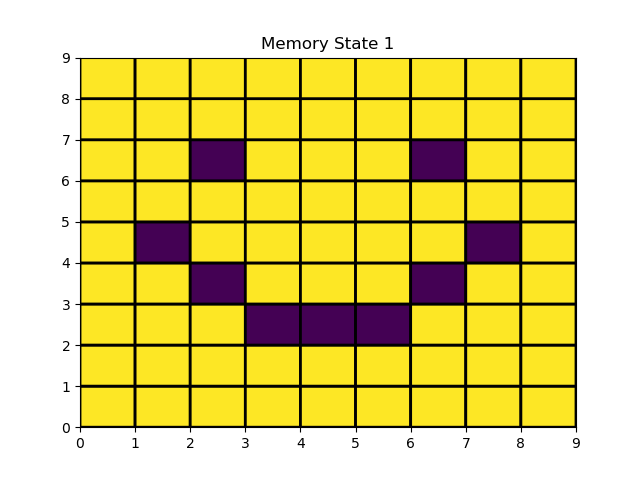
\includegraphics[scale = 0.3]{state_9x9_1.png}
\column{.5\textwidth}
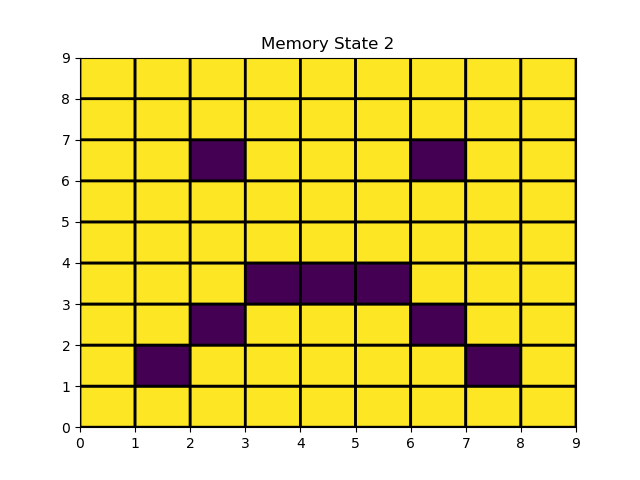
\includegraphics[scale = 0.3]{state_9x9_2.png}
\end{columns}
\item Se ejecutarán 11 simulaciones desde el mismo estado inicial aleatorio para distintos valores de $T$. El número de steps será siempre 100000.

\end{itemize}   
\end{frame}

\begin{frame}
\frametitle{Simulación de Montecarlo}
\framesubtitle{Estados de Mattis}
Para $T = 0$
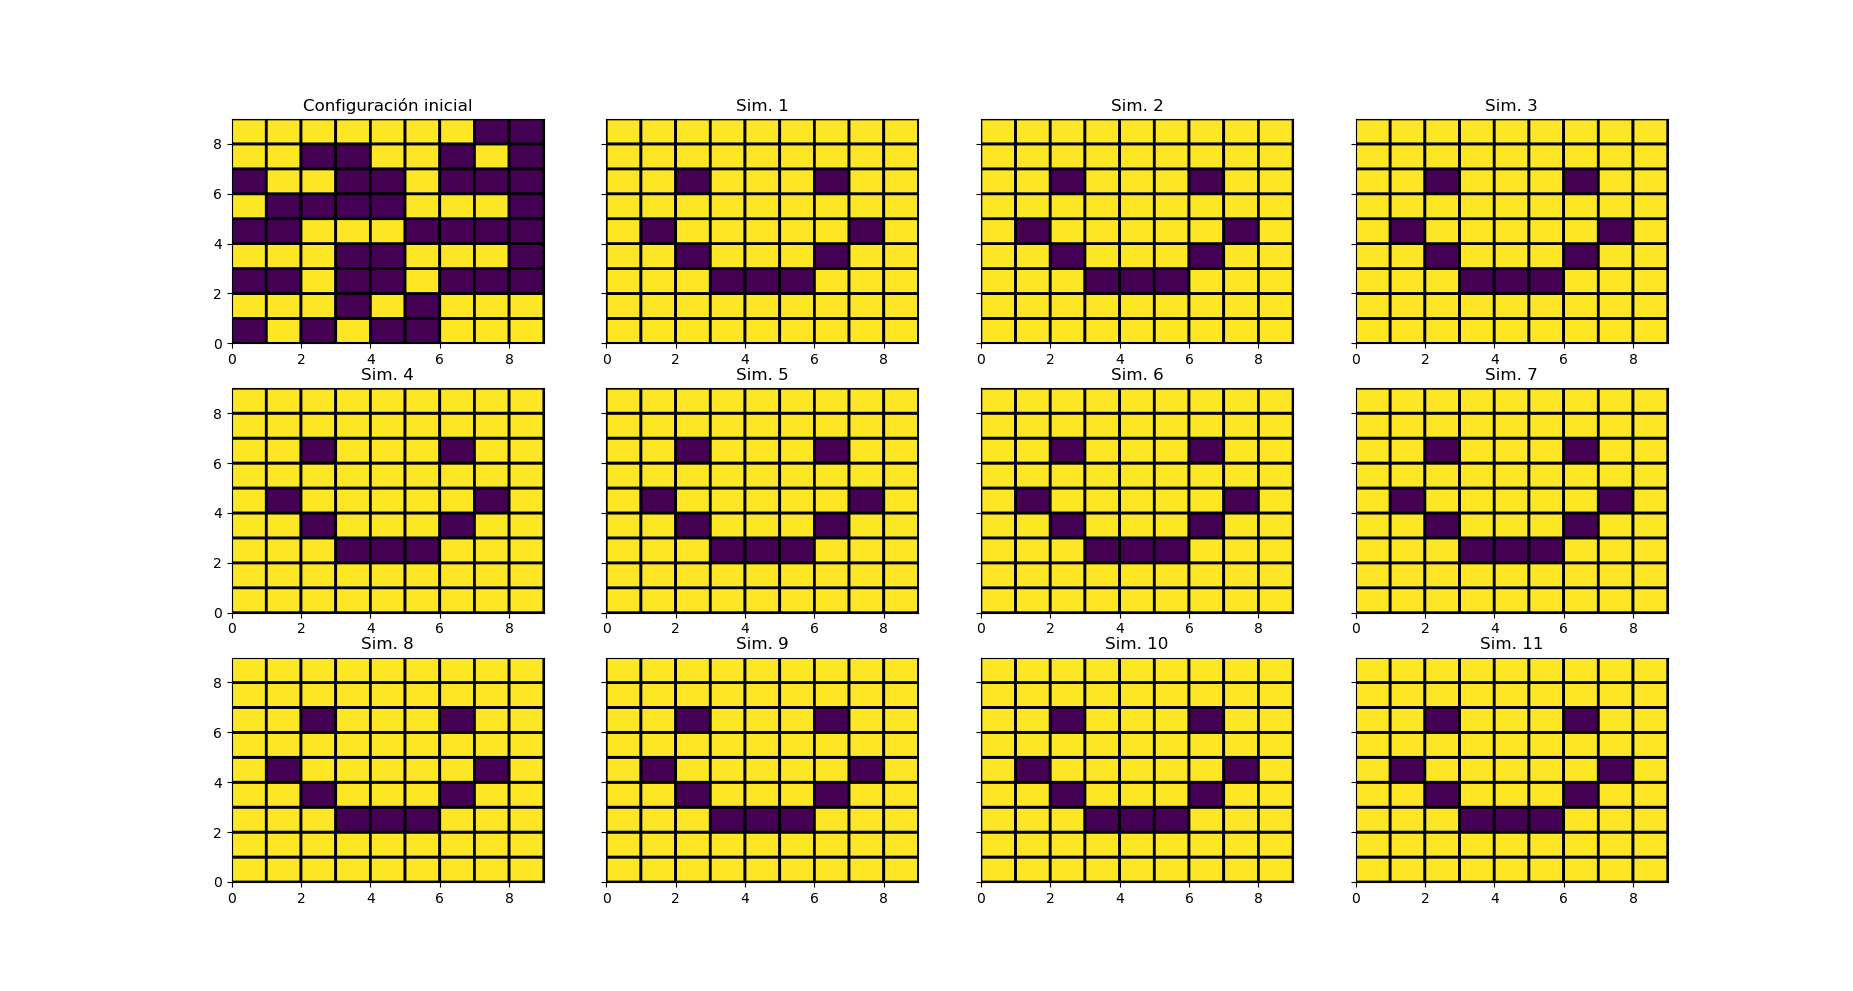
\includegraphics[width=\linewidth]{9x9_T=0.png}

\end{frame}

\begin{frame}
\frametitle{Simulación de Montecarlo}
\framesubtitle{Estados de Mattis}
Para $T = 0.2$
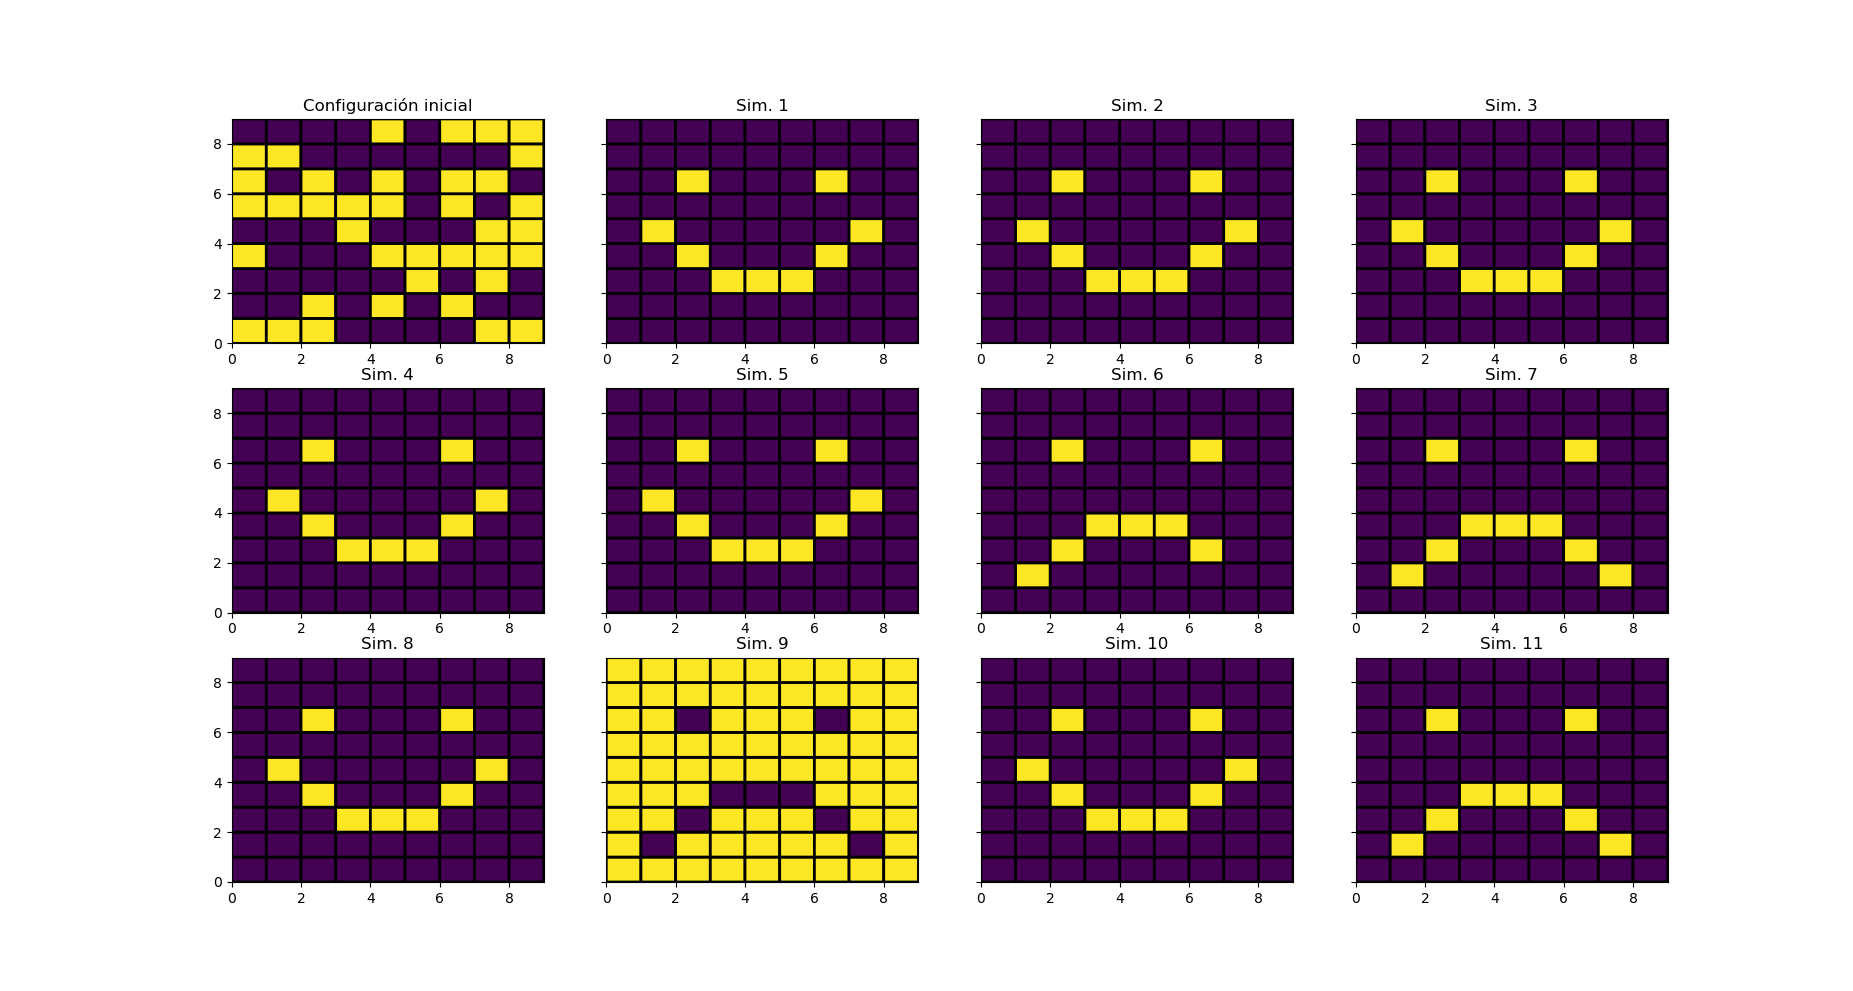
\includegraphics[width=\linewidth]{9x9_T=0,2.png}

\end{frame}

\begin{frame}
\frametitle{Simulación de Montecarlo}
\framesubtitle{Estados de Mattis}
Para $T = 0.5$
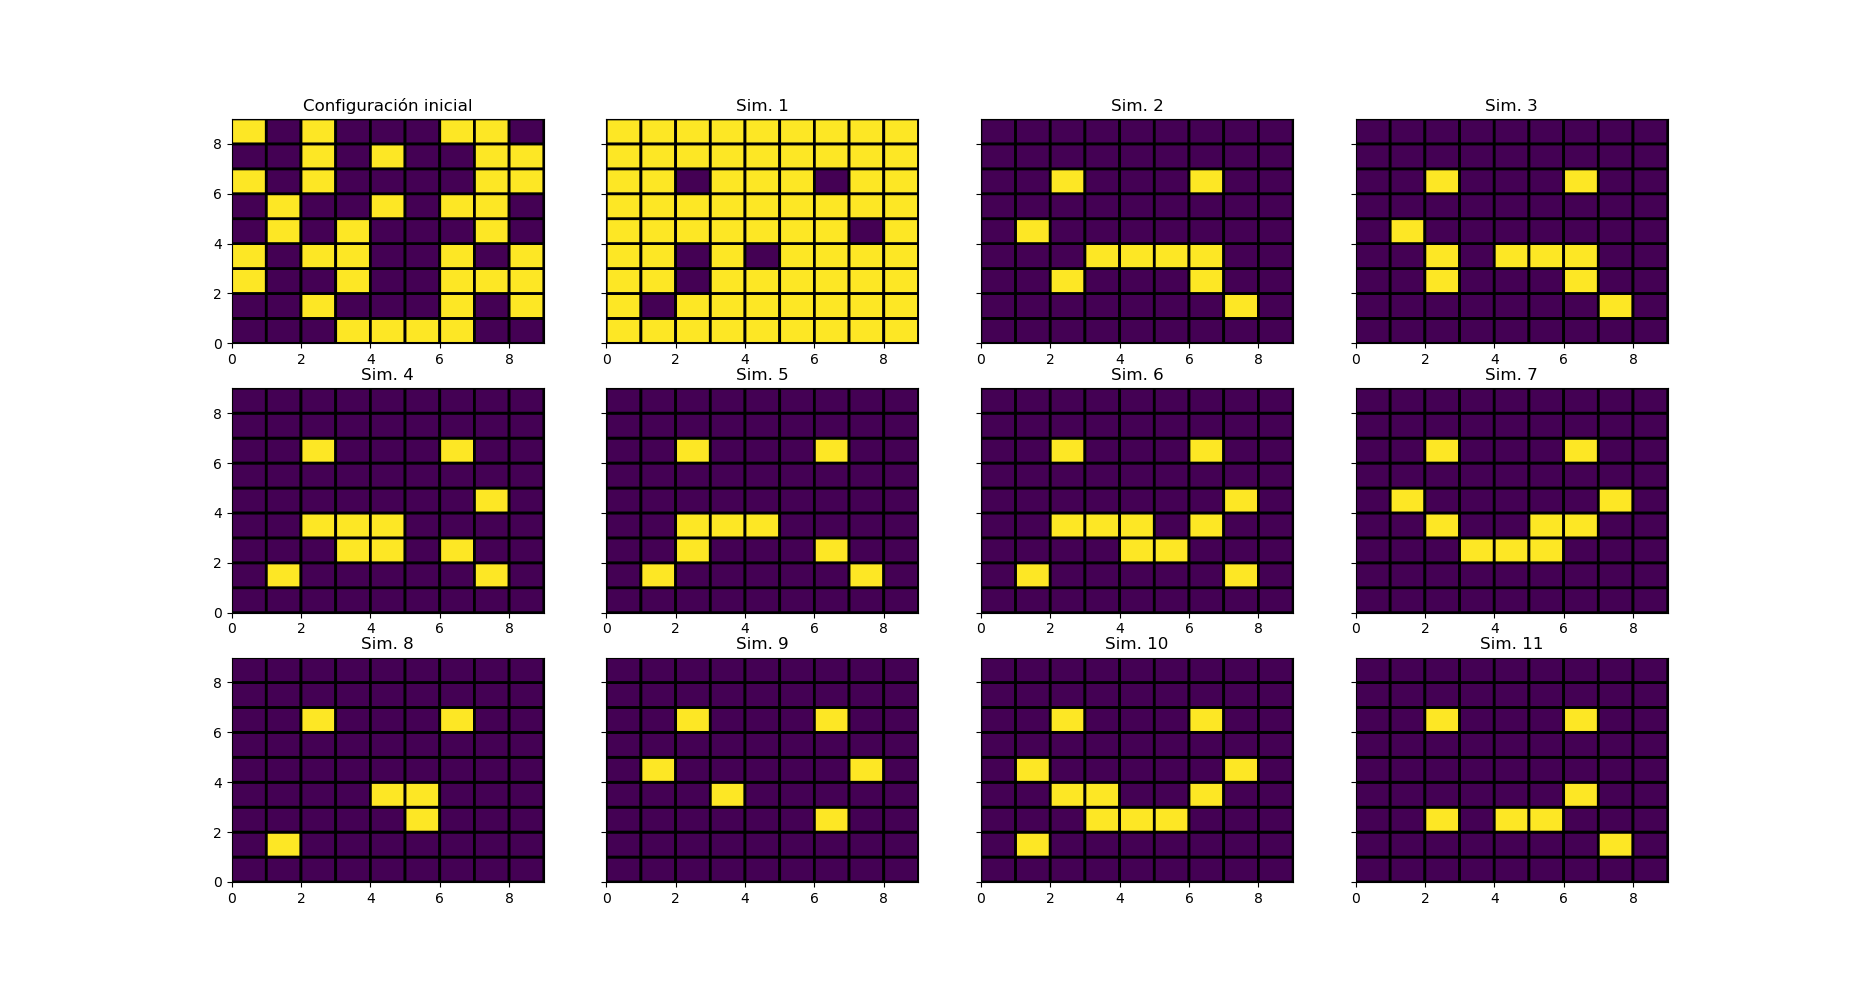
\includegraphics[width=\linewidth]{9x9_T=0,5.png}

\end{frame}

\begin{frame}
\frametitle{Simulación de Montecarlo}
\framesubtitle{Estados de Mattis}
Para $T = 1.2$
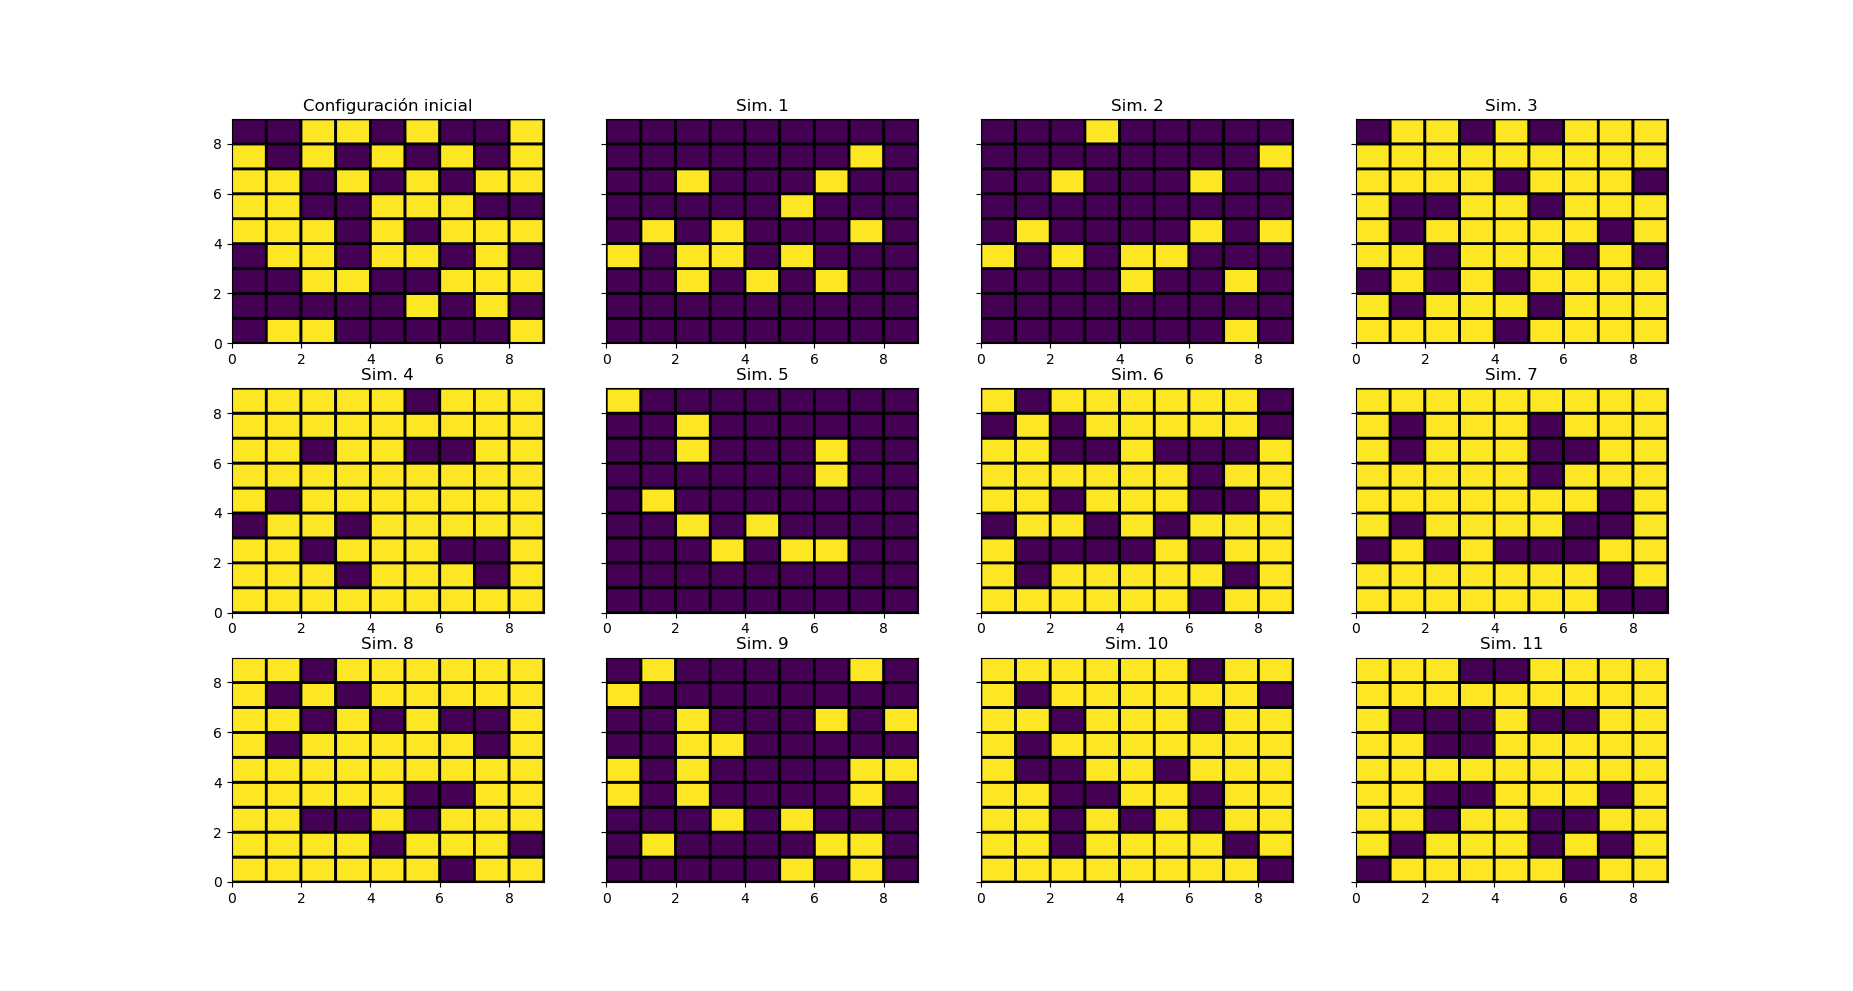
\includegraphics[width=\linewidth]{9x9_T=1,2.png}

\end{frame}

\begin{frame}
\frametitle{Simulación de Montecarlo}
\framesubtitle{Transición de fase}
\begin{itemize}
\item Comportamiento cerca de la temperatura crítica $T_{c} = 1$.
\item Parámetro de orden $\longrightarrow$ \textit{Overlap}
$$
m^{\mu} = N^{-1} \left| \sum_{i=1}^{N} \langle S_{i} \rangle \mathcal{P}^{\mu}_{i}  \right|
$$
\item Se utilizará sólo un estado de memoria para distintos tamaños de la red.
\end{itemize}
\end{frame}

\begin{frame}
\frametitle{Simulación de Montecarlo}
\framesubtitle{Transición de fase}
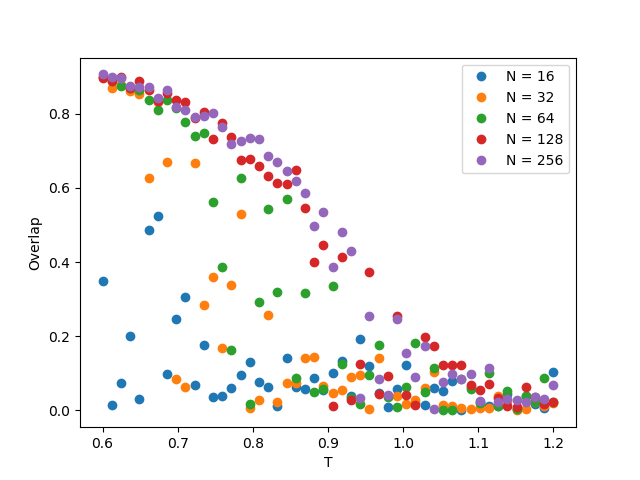
\includegraphics[width=\linewidth]{Overlap_FSS.png}
\end{frame}

\begin{frame}
\frametitle{Simulación de Montecarlo}
\framesubtitle{Transición de fase}
Observaciones:
\begin{itemize}
\item Difícil encontrar puntos donde se haya alcanzado el LT.
\item Cualitativamente $\longrightarrow$ Separación entre dos regiones: ordenada y caótica (no se guarda memoria).
\item Hipótesis $\longrightarrow$ No analiticidad en $T = 1$ en el LT $\longrightarrow$ Transición de segundo orden.
\end{itemize}
\end{frame}

\begin{frame}
\frametitle{Simulación de Montecarlo}
\framesubtitle{Estados metaestables}
\begin{itemize}
\item Red cuadrada $10 \times 10$ ($N = 100$).
\item Tres estados de memoria:
\begin{columns}
\column{.33\textwidth}
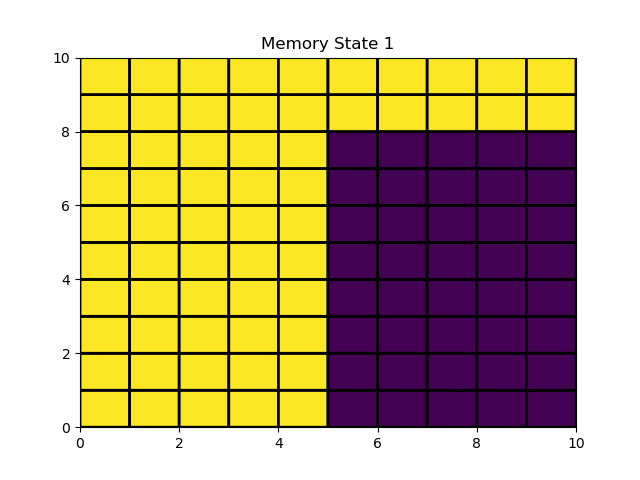
\includegraphics[width=\linewidth]{state_10x10_1.png}
\column{.33\textwidth}
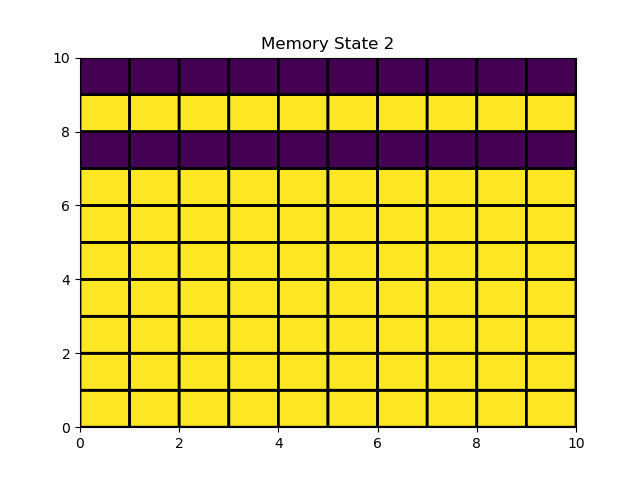
\includegraphics[width=\linewidth]{state_10x10_2.png}
\column{.33\textwidth}
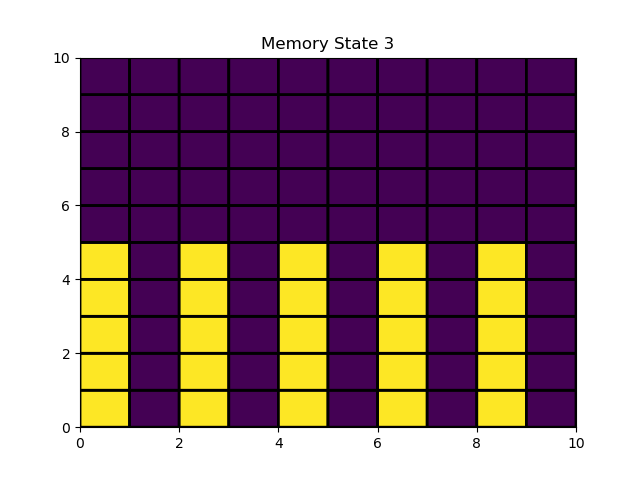
\includegraphics[width=\linewidth]{state_10x10_3.png}
\end{columns}
\item Para cada simulación se representa la evolución del módulo de la \textit{magnetización} del sistema, así como su energía.
$$
|M|(\{ S\}) = N^{-1} \left| \sum_{i=1}^{N} S_{i} \right|
$$

\end{itemize}   
\end{frame}

\begin{frame}
\frametitle{Simulación de Montecarlo}
\framesubtitle{Estados metaestables}
Ejemplo para $T = 0$.
\begin{columns}
\column{.5\linewidth} 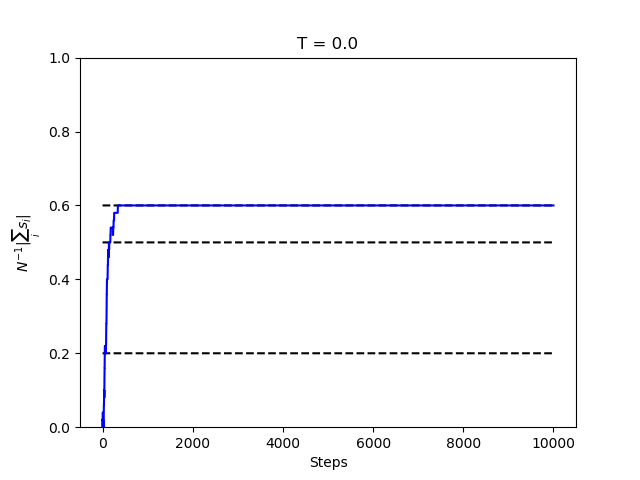
\includegraphics[width=\linewidth]{example_magnet.png}
\column{.5\linewidth} 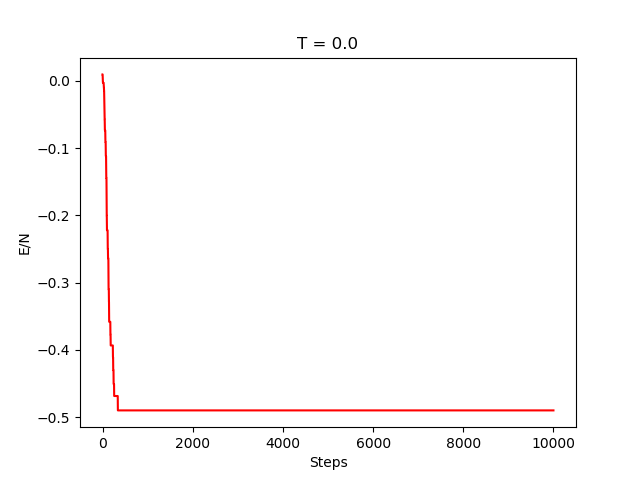
\includegraphics[width=\linewidth]{example_ener.png}
\end{columns}
\end{frame}

\begin{frame}
\frametitle{Simulación de Montecarlo}
\framesubtitle{Estados metaestables}
Estado metaestable para $T = 0$.
\begin{columns}
\column{.5\linewidth} 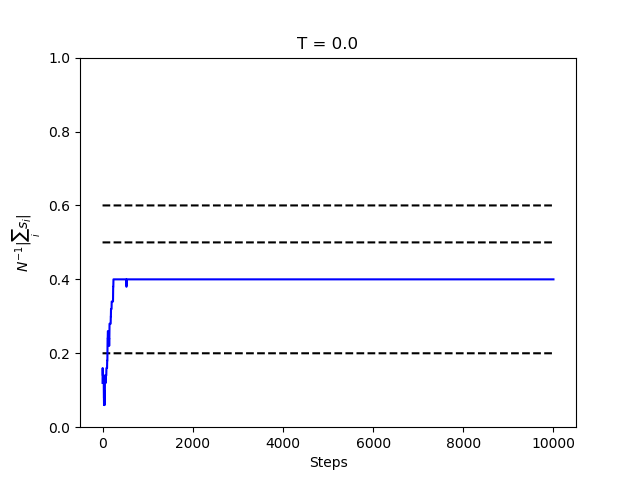
\includegraphics[width=\linewidth]{magnet_meta_T=0,0.png}
\column{.5\linewidth} 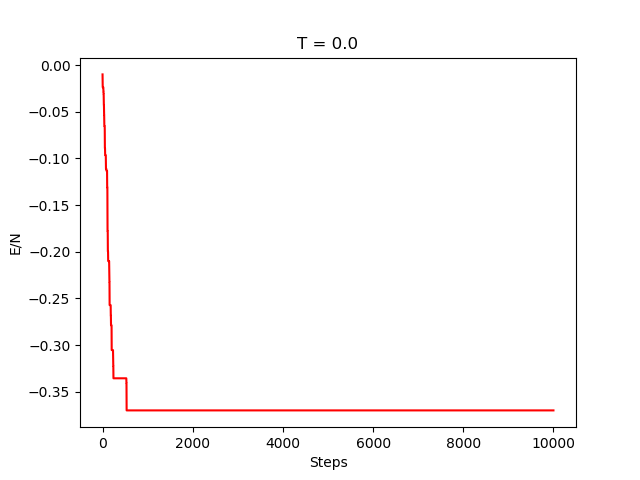
\includegraphics[width=\linewidth]{ener_meta_T=0,0.png}
\end{columns}
\end{frame}

\begin{frame}
\frametitle{Simulación de Montecarlo}
\framesubtitle{Estados metaestables}
Estado metaestable para $T = 0$.
\begin{columns}
\column{.5\linewidth} 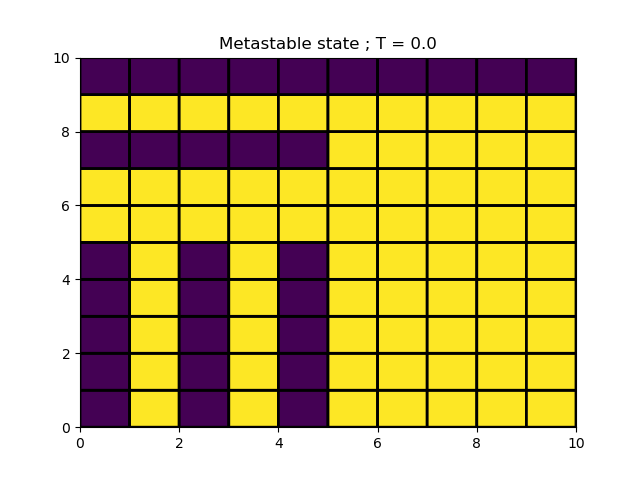
\includegraphics[width=\linewidth]{meta_T=0,0.png}
\column{.5\linewidth} 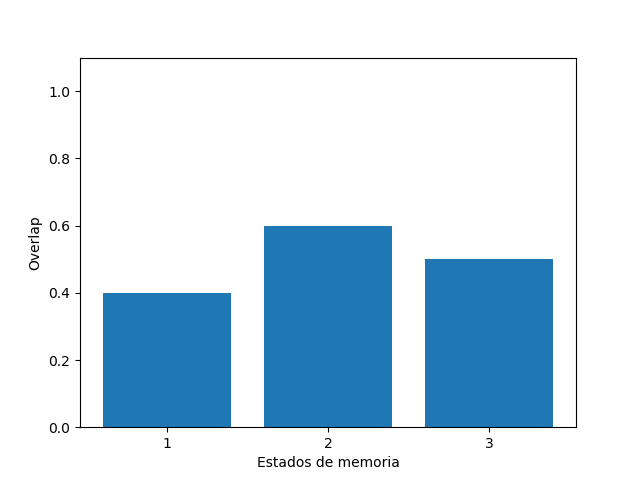
\includegraphics[width=\linewidth]{Metastable_overlap.png}
\end{columns}
\end{frame}

\begin{frame}
\frametitle{Simulación de Montecarlo}
\framesubtitle{Estados metaestables}
Estado metaestable para $T = 0.1$.
\begin{columns}
\column{.5\linewidth} 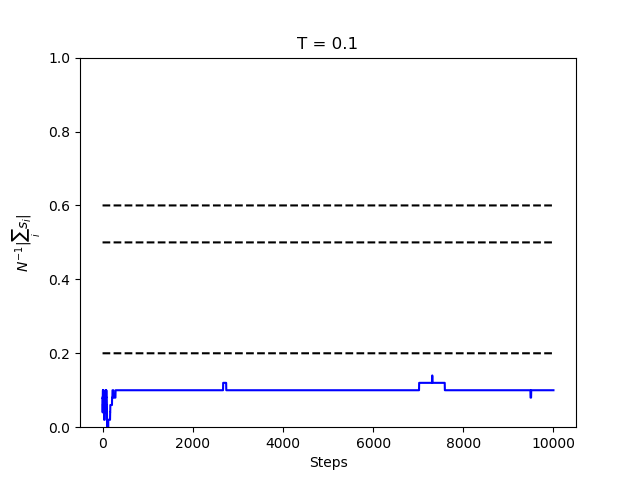
\includegraphics[width=\linewidth]{magnet_meta_T=0,1.png}
\column{.5\linewidth} 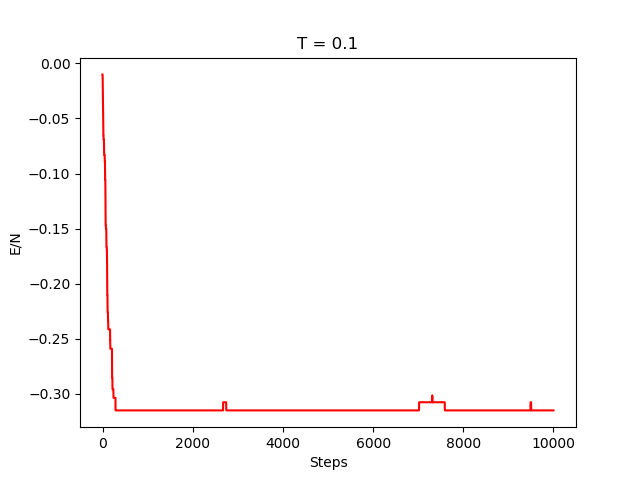
\includegraphics[width=\linewidth]{ener_meta_T=0,1.png}
\end{columns}
\end{frame}

\begin{frame}
\frametitle{Simulación de Montecarlo}
\framesubtitle{Estados metaestables}
Estado metaestable para $T = 0.2$.
\begin{columns}
\column{.5\linewidth} 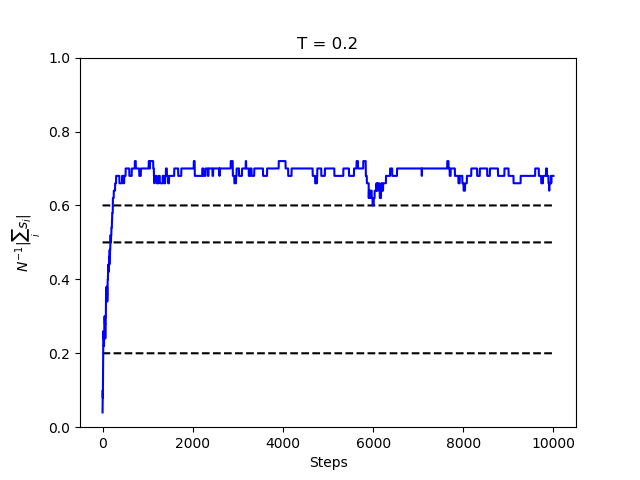
\includegraphics[width=\linewidth]{magnet_meta_T=0,2.png}
\column{.5\linewidth} 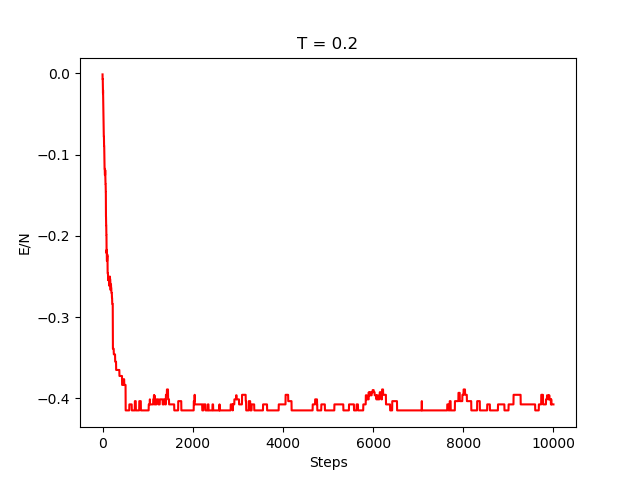
\includegraphics[width=\linewidth]{ener_meta_T=0,2.png}
\end{columns}
\end{frame}

\begin{frame}
\frametitle{Simulación de Montecarlo}
\framesubtitle{Estados metaestables}
\begin{columns}
\column{.5\linewidth}
Estado metaestable para $T = 0.1$.
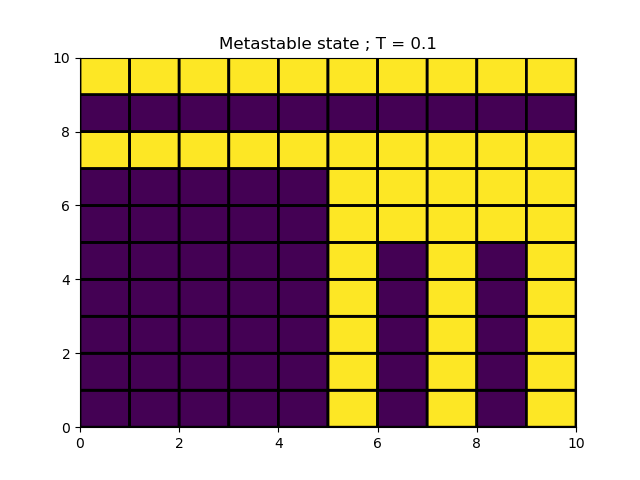
\includegraphics[width=\linewidth]{meta_T=0,1.png}
\column{.5\linewidth}
Estado metaestable para $T = 0.2$.
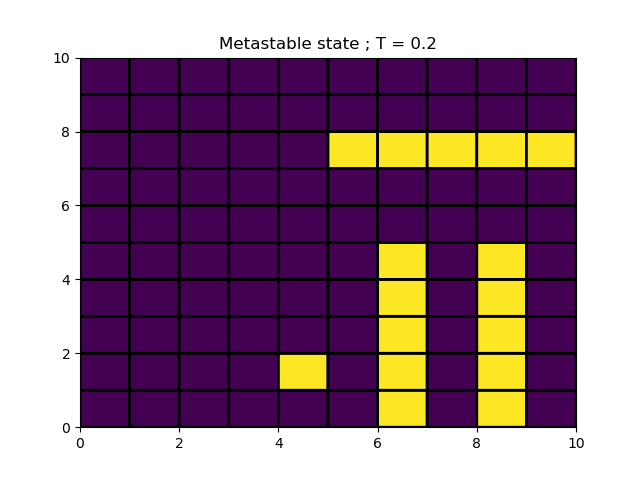
\includegraphics[width=\linewidth]{meta_T=0,2.png}
\end{columns}
\end{frame}


\begin{frame}
\frametitle{Ecuación de Langevin}
\framesubtitle{Formulación continua}
\begin{itemize}
	\item Necesitamos que $\sigma_i \rightarrow \pm 1$ conforme $t \rightarrow \infty$
	\item Incluimos fluctuaciones térmicas con $\xi_i(t)$
	\item Fluctuaciones independientes $\langle \xi_i(t) \xi_j(t') \rangle = 2T\delta(t-t')\delta_{ij}$
	\begin{displaymath}
	\frac{\partial\sigma_i}{\partial t} = -\lambda(\sigma_i^2-1)\sigma_i + \sum_j J_{ij}\sigma_j + h_i\sigma_i + \xi_i(t)
	\end{displaymath}	
\end{itemize}
\end{frame}
\begin{frame}
\frametitle{Ecuación de Langevin}
\framesubtitle{Formulación discreta}
\begin{itemize}
	\item Diferencial estocástico $\mu(dW_i) = 0, \sigma^2(dW_i) = dt$
	\begin{displaymath}
	d\sigma = \left( -\lambda(\sigma_i^2 - 1)\sigma_i +  \sum_j J_{ij} \sigma_j + h_i\sigma_i \right) dt + \sqrt{2T}dW_i
	\end{displaymath}	
\end{itemize}
\end{frame}

\begin{frame}
\frametitle{Ecuación de Langevin}
\framesubtitle{Valor de $\lambda$}
\begin{itemize}
	\item Valores demasiado grandes de $\lambda$ hacen que no haya evolución
	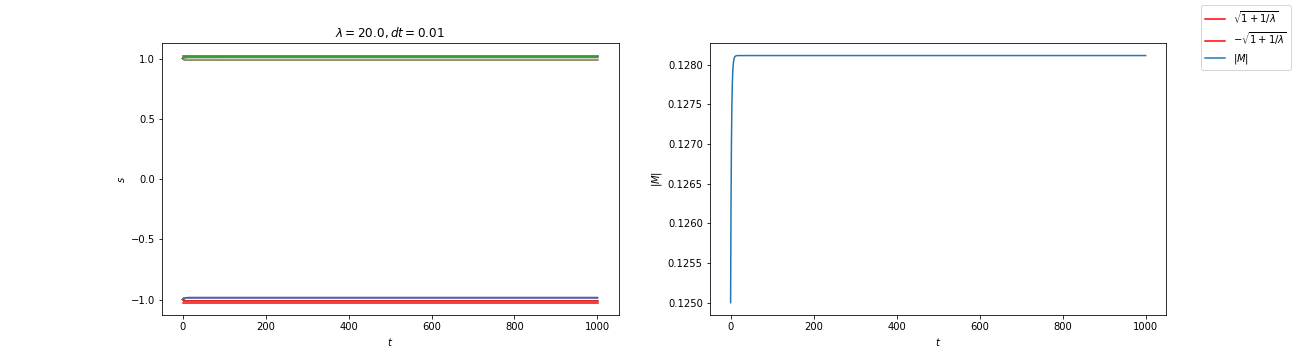
\includegraphics[width=\linewidth]{Sobreamortiguado.png}
	\item Valores demasiado grandes de $\lambda$ hacen no se acerce a $\pm 1$
	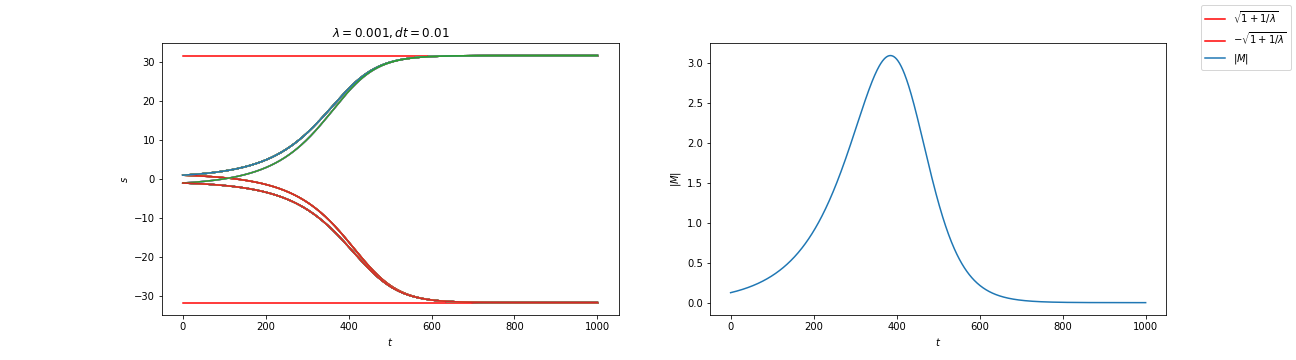
\includegraphics[width=\linewidth]{Subamortiguado.png}
\end{itemize}
\end{frame}

\begin{frame}
\frametitle{Ecuación de Langevin}
\framesubtitle{Valor de $\lambda$}
\begin{itemize}
	\item Valores cercanos a 1 dan una evolución razonable
	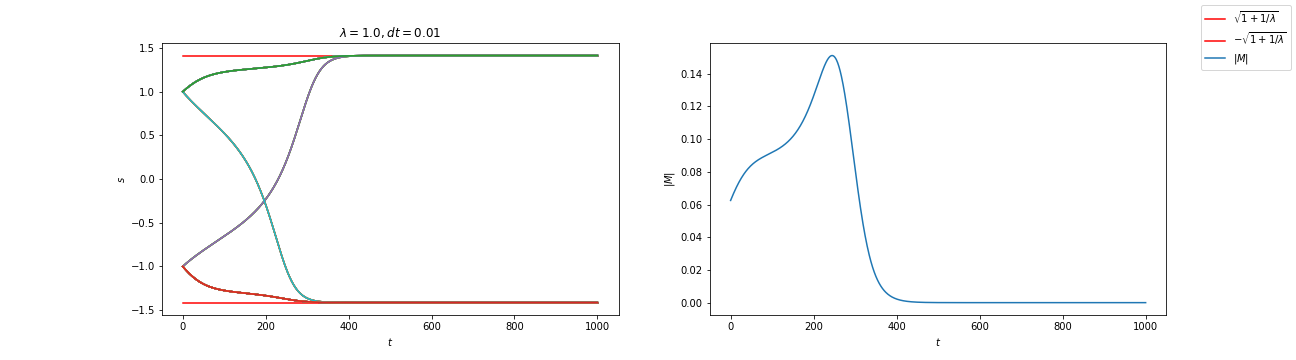
\includegraphics[width=\linewidth, trim= 0 0 0 -3cm]{Normal.png}
\end{itemize}
\end{frame}

\begin{frame}
\frametitle{Ecuación de Langevin}
\framesubtitle{Resultados}
\begin{itemize}
	\item El sistema evoluciona a los estados ``guardados'' en  $J_{ij}$\\
	\centering
	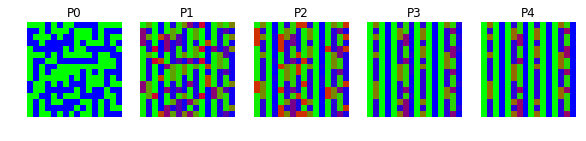
\includegraphics[width=0.75\linewidth]{evolucion_langevin-0.png}
	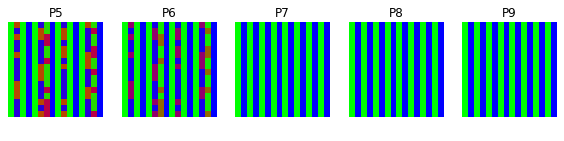
\includegraphics[width=0.75\linewidth]{evolucion_langevin-1.png}
	\item  $g(\sigma(t)) - \sigma(t) \rightarrow 0$ (condicion estacionaria)
	\centering
	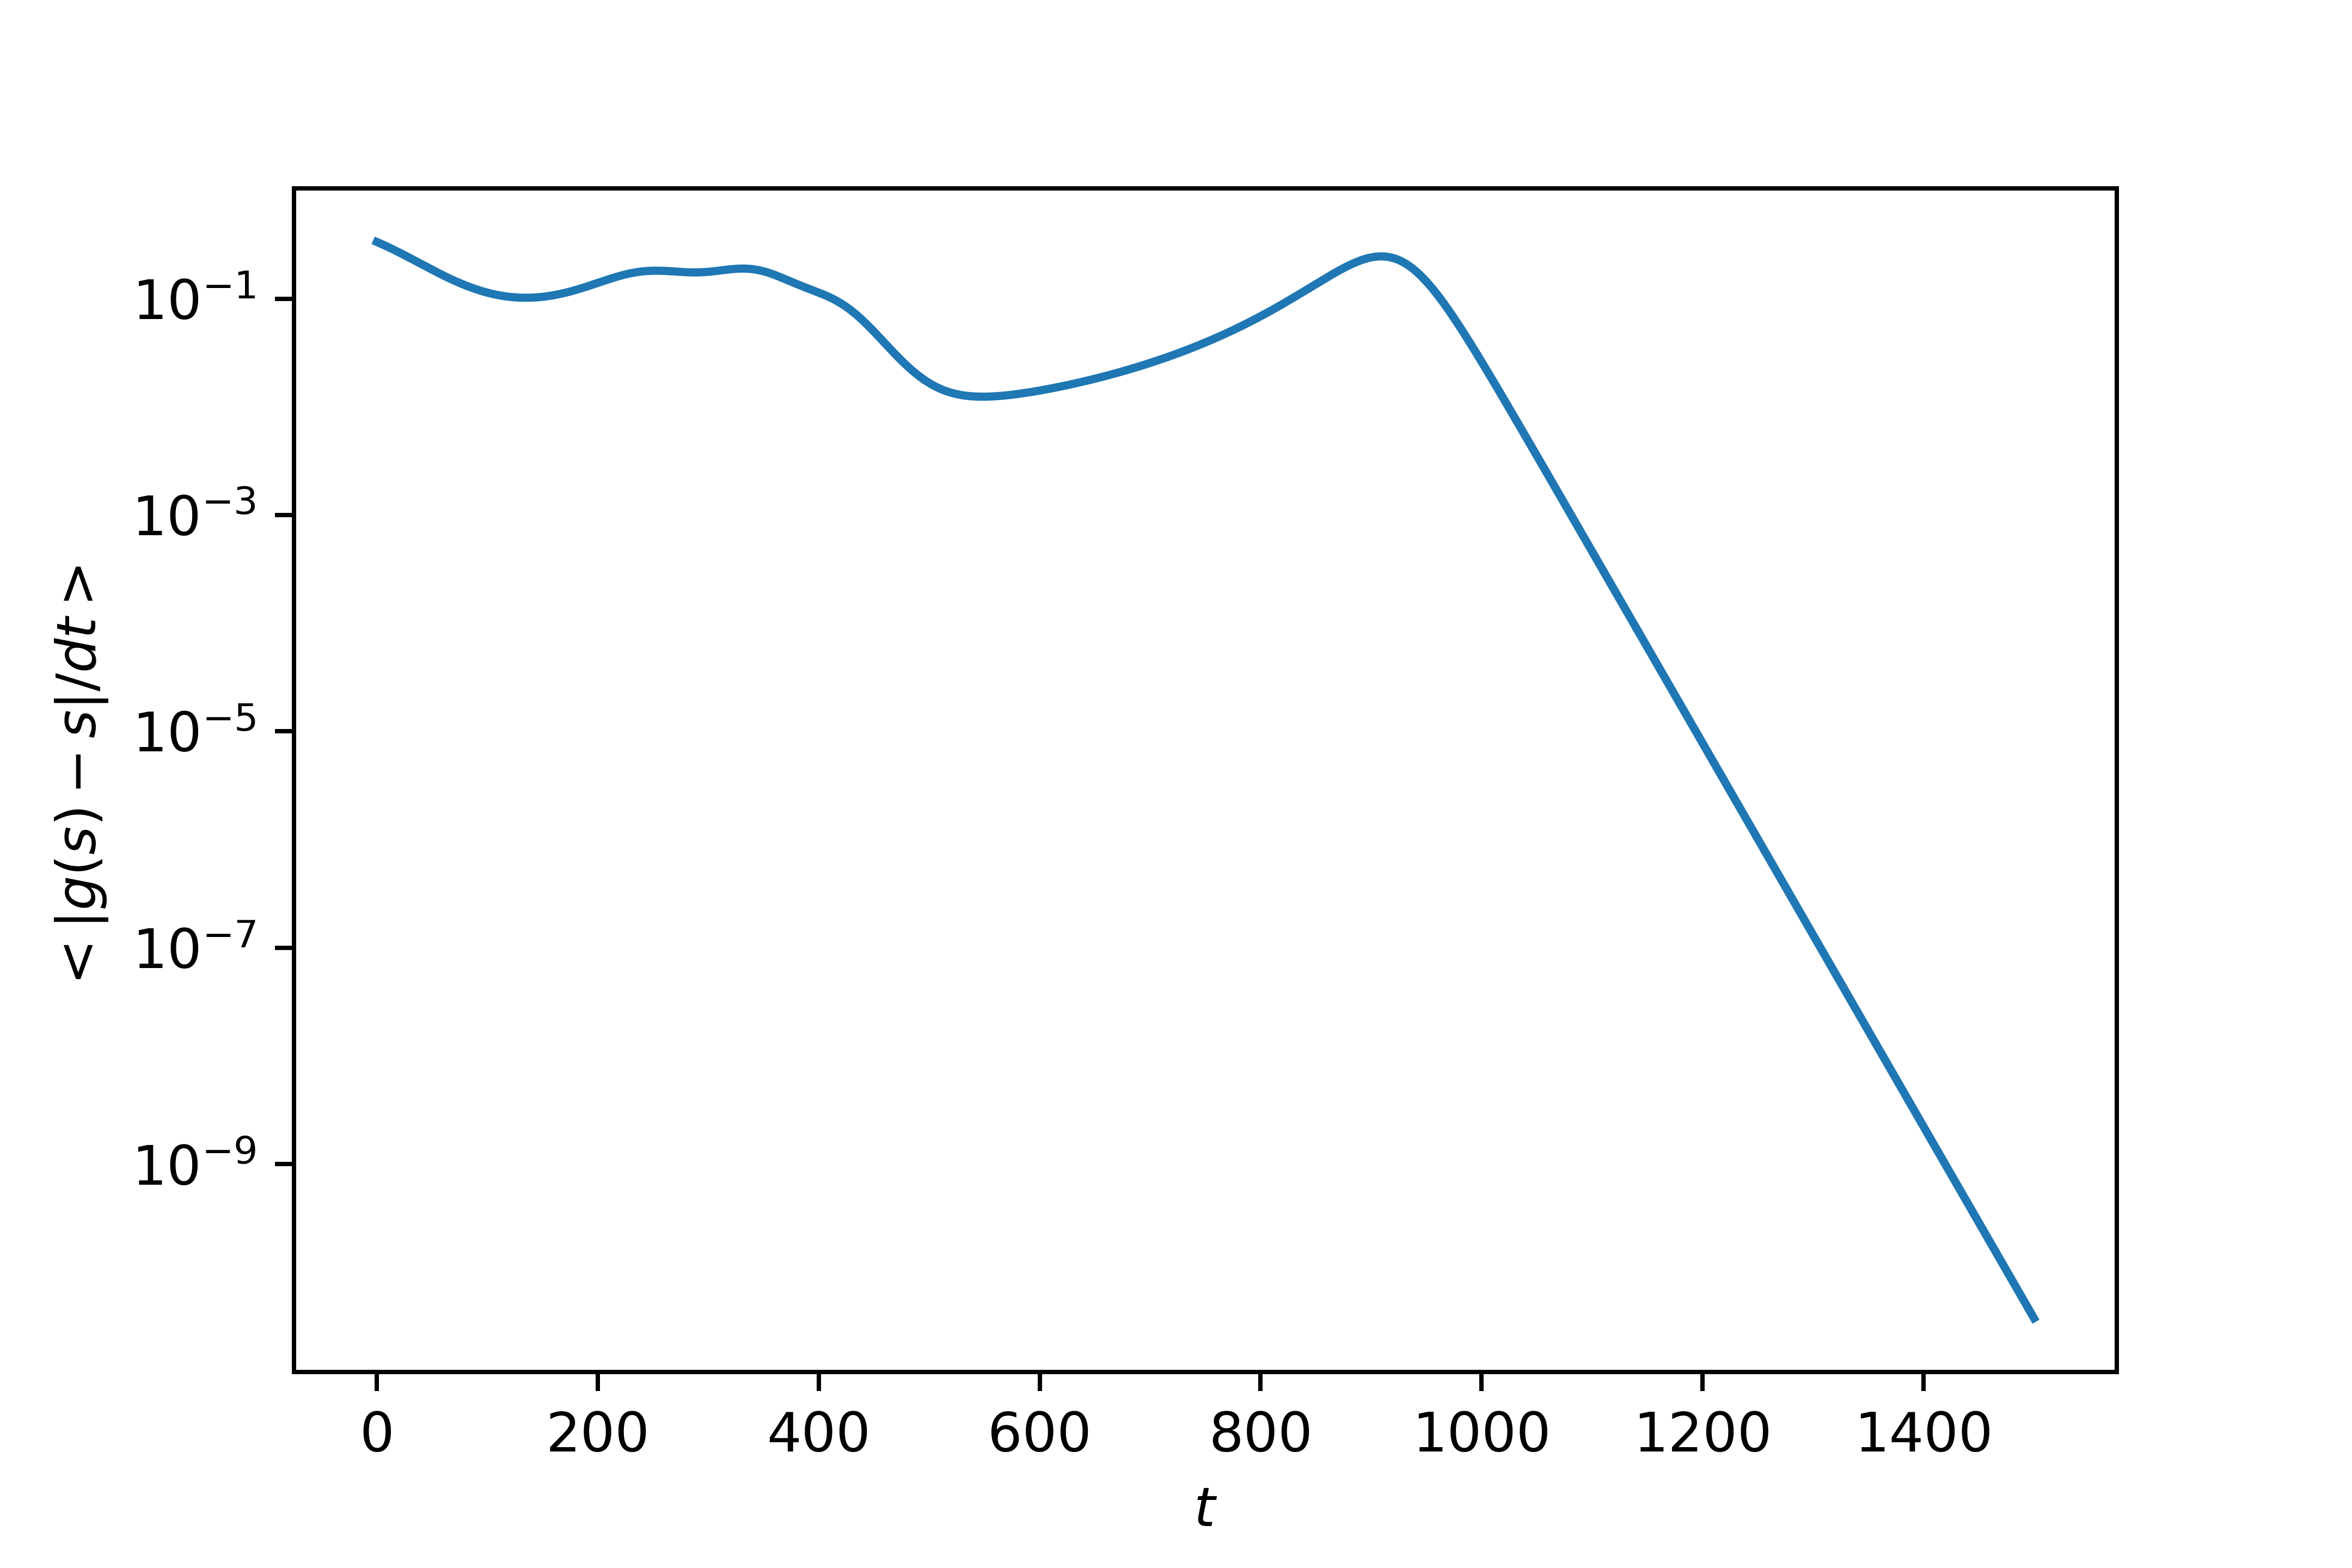
\includegraphics[width=0.45\linewidth]{convergencia_langevin.png}
\end{itemize}
\end{frame}

\end{document}
